\section{Straggling} \label{sec:ICOOLStraggling}
ICOOL \cite{icool} employs four levels of straggling models, three of which were used in these muon simulations studies. They are
\begin{enumerate}
\item{Gaussian (Bohr)},
\item{Landau distribution}, and
\item{Vavilov distribution (with appropriate limits)}.
\end{enumerate}
The fourth model is ``restricted energy fluctuations from continuous processes with energy below DCUTx" and was not used for this study.

\subsection{Gaussian (Bohr)} \label{ssc:ICOOLStragglingGaussian}

The first model uses a Guassian function to model the energy loss distribution. Recall that Gaussian distributions can be determined from two parameters: the mean $\mu$ and the standard deviation $\sigma$. The first of these comes from the Bethe Bloch equation, which will be derived here and yeilds Eqn. \ref{eqn:bethebloch}. 

%..........................................
\vspace{24pt}
\noindent \textit{\large Classical Derivation}
\vspace{12pt}

The model begins with a particle of charge $e$ moving into a volume of electrons. It is assumed that the mass of the incoming particle is much greater than the mass of the electron since there will be no scattering in this derivation. Moreover, the electron must either be at rest and fixed into place (which is nonphysical) or the collision time of the particle and electron is very small compared to the electron orbital time. The $z-$axis is aligned with the particle's velocity such that $v_x=v_y=0$. The momentum transfer $\Delta p$ is sought, and the first observation is that the change in longitidunal momentum is zero (i.e. $\Delta p_z=0$). This is true since the particle feels a force ``forwards" just as much as it feels a force ``backwards". Since this model bars scattering, the change in momentum must be interpreted as energy imparted upon the electron. Then:
\begin{align*}
\Delta p_x &=\int_{-\infty} ^\infty F_x dt = \int_{-\infty} ^{\infty} F_x \frac{dz}{v} = \int_{-\infty} ^{\infty} F\cos{\theta}\frac{dz}{v} \\
&= \int_{-\infty} ^{\infty} \frac{e^2}{r^2} \frac{b}{r} \frac{dz}{v} = \int_{-\infty} ^{\infty} \frac{e^2}{z^2+b^2} \frac{b}{\sqrt{z^2+b^2}} \frac{dz}{v}\\
&= \frac{e^2 b}{v} \int_{-\infty} ^{\infty} \frac{1}{(z^2+b^2)^{3/2}}dz,
\end{align*}
where $b$ is the impact parameter (the closest distance between the particle and the electron). By substitution of the following
\begin{align*}
z &= b\tan{\theta}\\
dz &= b\sec^2{\theta} d\theta\\
z=\infty&\rightarrow \theta = \frac{\pi}{2}\\
z=-\infty&\rightarrow \theta = \frac{-\pi}{2}
\end{align*}
the integral becomes
\begin{align*}
\Delta p_x &=\frac{e^2 b}{v}\int_{-\pi/2} ^{\pi/2} \frac{b\sec^2{\theta} d\theta}{(b^2(\tan^2{\theta}+1))^{3/2}}\\ &=\frac{e^2 b}{v}\int_{-\pi/2} ^{\pi/2} \frac{d\theta}{b^2 |\sec{\theta}|}\\
&=\frac{2e^2}{vb}.
\end{align*}

The non-relativistic approach yeilds the energy loss for the interaction between a muon and a single electron:
\begin{equation}\label{eqn:BetheBlochDeltaE}
\epsilon=\frac{\Delta p^2}{2m_e}=\frac{2e^4}{v^2 b^2 m_e}
\end{equation}
Here, it is useful to note that if the interaction of the muon with the nucleus was desired, $\epsilon$ for a single interaction would be proportional to $Z^2/m_{nuc}$ and would be added on to the above term. However, since $1/m_e >> 1/m_{nuc}$ the second term will be disregarded.

For multiple electrons, the average electron density is $N_{el}=N_A\cdot Z\rho/A$. The cylindrical symmetry of the system is exploited by integrating the single electron interaction in cylidrical coordinates, with the cylindrical angle as $\theta$, radius as $b$ (the impact parameter), and length as $z$. The bounds on $b$ are some $[b_{min},b_{max}]$ which will be discussed shortly. Then
\begin{align}
\left<\epsilon\right>&=\int_{b_{min}} ^{b_{max}} \int_0 ^L \int_0 ^{2\pi}  \frac{2e^4}{v^2b^2m_e}N_{el}\: d\theta \: dz\: b \,db \nonumber\\
&=\frac{4\pi N_A e^4}{v^2 m_e}\frac{Z\rho L}{A}\int_{b_{min}} ^{b_{max}} \frac{db}{b} \label{eqn:BetheBlochIntermediate}
\end{align}

It is known that $b_{min}$ comes from the maximum amount of enery ($T_{max}$) which a muon may impart upon an electron. This quantity is derived later and can be seen in Eqn. \ref{eqn:tmax}, but is only symbolic here. Similarly, the minimum transferrable energy is simply the (mean) ionization energy, $I$, which is usually taken as an emperical value. Any energy below this value will not transfer, since this is the minimum amount of energy to free the electron from its orbit. Then
\begin{align*}
\epsilon_{max}&=\frac{2e^4}{v^2b_{min} ^2 m_e}=T_{max}\\
b_{min}&=\frac{e^2}{v}\sqrt{\frac{2}{m_e T_{max}}}\\[12pt]
\epsilon_{min}&=\frac{2e^4}{v^2b_{max} ^2 m_e}=T_{min}=I\\
b_{max}&=\frac{e^2}{v}\sqrt{\frac{2}{m_e I}}.
\end{align*}

Now that the bounds have been acquired, the integral in Eqn. \ref{eqn:BetheBlochIntermediate} is solvable.
\begin{align}
\left<\epsilon\right> &= \frac{4\pi N_A e^4}{v^2 m_e} \frac{Z\rho L}{A}\int_{b_{min}} ^{b_{max}} \frac{db}{b}\nonumber\\
\left<\epsilon\right> &= \frac{4\pi N_A e^4}{v^2 m_e} \frac{Z\rho L}{A} \ln{\frac{b_{max}}{b_{min}}}\nonumber\\
\left<\epsilon\right> &= \frac{2\pi N_A e^4}{v^2 m_e} \frac{Z\rho L}{A} \ln{\frac{T_{max}}{I}} \label{eqn:BetheBlochClassical}.
\end{align}

%..........................................
\vspace{24pt}
\noindent \textit{\large{Modern Derivation}}
\vspace{12pt}

While Eqn. \ref{eqn:BetheBlochClassical} is a good start, there are many aspects which were not considered. The most obvious of these are the wavelike nature of the incoming muon, relativistic kinetic energy (not simply $p^2/2m$), and the relativistic flattening of the muon's electric field just to name a few. Therefore, a more rigorous derivation will be done with corrections added onto it.

Firstly, let the incoming muon be considered also a wave. Then the corresponding differential cross section $d\Sigma$ is defined as the area in which the muon loses an amount of energy between $\epsilon$ and $\epsilon+d\epsilon$. Given the impact parameter $b$, for a single electron this area is a ring of radius $b$ and thickness $db$, or \cite{bichsel1968,bichsel1988}
\begin{align*}
d\Sigma=2\pi b \, db.
\end{align*}
Using the result from Eqn. \ref{eqn:BetheBlochDeltaE} in the classical derivation, this becomes
\begin{align*}
\epsilon &= \frac{2e^4}{\beta^2 b^2 m_e}\\
b^2 &= \frac{2e^4}{\beta^2 \epsilon m_e}\\
2b \, db &= -\frac{2e^4}{\beta^2 \epsilon^2 m_e}d\epsilon,
\end{align*}
and so
\begin{align*}
d\Sigma=\frac{2\pi e^4}{\beta^2} \frac{d\epsilon}{\epsilon ^2}.
\end{align*}
The relativistic correction for this was calculated by Bhabha \cite{uehling,bhabha} and results in
\begin{align*}
d\Sigma=\frac{2\pi e^4}{\beta^2} \frac{d\epsilon}{\epsilon ^2}\Big(1-\frac{\beta^2 \epsilon}{T_{max}}\Big).
\end{align*}
Note that in \cite{uehling}, this result is only for spin-0 particles, and there is a further correction factor of $\epsilon ^2 / 2E^2$ for spin-1/2 particles. However, since $E>>\epsilon$ this term is usually ignored.

The cross section may now be used in the standard definition of moments (or expectation values). Then
\begin{align} \label{eqn:StragglingMoments}
\left<\epsilon^j\right>&=N_{el} L \int_{\epsilon_{min}} ^{\epsilon_{max}} \epsilon^j \frac{d\Sigma}{d\epsilon} d\epsilon .
\end{align}
It is interesting to note that the zeroth moment is the mean number of collisions, and that the actual number of collisions is sampled from a Poisson distribution with this average. Moreover, $\left<\epsilon^1\right>$ is the mean energy loss, which is the desired outcome of this derivation. Then
\begin{align*}
\left<\epsilon\right>&=\frac{Z\rho L}{A} \frac{2\pi e^4}{\beta^2} \int_I ^{T_{max}} \frac{d\epsilon}{\epsilon} \Big(1-\frac{\beta^2 \epsilon}{T_{max}}\Big)\\
\left<\epsilon\right>&=\frac{Z\rho L}{A} \frac{2\pi e^4}{\beta^2} \Big(\ln{\frac{T_{max}}{I}}-\beta^2 (1-\frac{I}{T_{max}})\Big)
\end{align*}







In its more familiar form, the constants in front are condensed into a single constant $K=\frac{2\pi e^4 N_A}{m_e}\approx 15.4$ $ (\text{MeV}\cdot \text{cm}^3)/(\text{m}\cdot \text{g})$. Since the model assumes natural units of light (i.e. $\text{c}=1$), $v^2$ is usually replaced with $\beta ^2$. Moreover, to avoid confusion $\left<\epsilon\right>$ is given a negative sign in order to emphasize energy \emph{loss}.

There are a number of corrections to the Bethe-Bloch equation.The first is a correction under the logarithm due to the relativistic flattening of the incoming particle's electric field. This factor is  $2m_e \beta^2 \gamma^2 / I$. Another correction is known as the density correction parameter $\delta$ and arises due to polarization. This is important for high energies and may or may not be useful for these medium energy studies. The last correction is the shell correction parameter $C$ and accounts for the fact that the electron is not at rest (or the interaction time is not much faster than the electron orbit). This is important for low energies and may or may not be useful for these medium energy studies.

The final result is the Bethe-Bloch equation for the average energy lost by a particle traversing some medium with correction factors (with correction factors according to \cite{cosy}:
\begin{equation}\label{eqn:bethebloch}
\left< \epsilon \right> = -\frac{K}{\beta^2}\frac{Z\rho L}{A}\Big(\ln{\frac{2m_e \beta ^2 \gamma ^2 T_{max}}{I^2}}-2\beta^2-\delta-2\frac{C}{Z}\Big).
\end{equation}

According to the Particle Data Group \cite{PDG}, this equation is generally accurate for intermediate $Z$ materials (up to a few \% when compared to experimental data) in the energy regime of $0.1 \lesssim \beta \gamma \lesssim 1000$. The lower limit of this equation is when the incoming particle's velocity is comparable to the atomic electron velocities and the upper limit is due to radiative effects, as well as both limits having some $Z$ dependence. Figure \ref{fig:bethecurve} depicts this region approximately with muons on copper. Clearly, the region for muon ionization cooling ($100 \text{MeV/c} < p_\mu < 1000 \text{MeV/c}$) falls in the middle of the Bethe region, with the Anderson-Ziegler region as the low cutoff and radiative losses coming into effect at the high cutoff.

As previously stated, the first energy loss model from ICOOL selects an energy loss from a Gaussian profile with mean $\mu=\left<\epsilon \right>$ (Eqn. \ref{eqn:bethebloch}) and standard deviation according to \cite{geant4}:
\begin{equation}\label{eqn:bohrvariance}
\sigma^2=2\pi e^2 N_A T_c \frac{Z\rho L}{A} \frac{1-\beta^2/2}{\beta},
\end{equation}
where $T_c$ is the cut kinetic energy of $\delta$-electrons.

%..........................................
\vspace{24pt}
\noindent \textit{\large{Derivation of $T_{max}$}}
\vspace{12pt}

Although $T_{max}$ does have symbolic meaning in many equations, here it will be derived explicitly from a relativistic point of view. This derivation yields Eqn. \ref{eqn:tmax} and works in natural light units such that $\text{c}=1$. Conservation of energy for a muon incident upon an electron at rest requires that 
\begin{align}
E_\mu+m_e&=E_{\mu,f}+E_e,&\text{ or} \nonumber\\
\sqrt{p_\mu ^2+m_\mu ^2}+m_e &= \sqrt{p_{\mu,f}^2+m_\mu ^2}+T_e+m_e,&\text{ or} \nonumber \\
p_{\mu,f}^2 =p_\mu^2 &+T_e^2-2T_e\sqrt{p_\mu ^2 + m_\mu^2} \label{eqn:TMaxEnergy1}
\end{align}
with
\begin{align}
E_e=T_e&+m_e = \sqrt{p_e ^2+m_e^2},\qquad\text{ or} \nonumber\\
p_e ^2&=(T_e+m_e)^2-m_e^2 \label{eqn:TMaxEnergy2}
\end{align}
where $T_e$ is the final kinetic energy of the electron, $p_\mu$ is the initial muon momentum, $m_\mu$ is the mass of the muon, and $p_{\mu,f}$ is the final muon momentum. 

Conservation of momentum requires that
\begin{align*}
\vec{p}_\mu&=\vec{p}_{\mu,f}+\vec{p}_e, \qquad\text{ or}\\
 p_{\mu,f}^2&=p_\mu ^2 + p_e^2-2p_\mu p_e \cos\theta.
\end{align*}
Using Eqn. \ref{eqn:TMaxEnergy2} for $p_e$ on the right side this becomes
\begin{align*}
p_{\mu,f}^2=p_\mu ^2+(T_e+m_e)^2-m_e ^2-2p_\mu\cos\theta \sqrt{(T_e+m_e)^2-m_e^2)}
\end{align*}
Now subsitution of Eqn. \ref{eqn:TMaxEnergy1} for $p_{\mu,f} ^2$ on the left side yields
\begin{align*}
p_\mu ^2+T_e ^2 - 2T_e \sqrt{p_\mu^2+m_\mu ^2}&=p_\mu ^2+(T_e+m_e)^2-m_e ^2 \sqrt{(T_e+m_e)^2-m_e^2)}
\end{align*}
For maximum energy (i.e. to attain $T_e=T_{max}$), $\cos\theta=1$, which is representative of a head-on collision. Then
\begin{align*}
T_{max} ^2-2T_{max}\sqrt{p_\mu ^2+m_\mu ^2} &=T_{max}^2+2T_{max}m_e-2p_\mu\sqrt{T_{max}^2+2T_{max}m_e}\\
-2T_{max}(\sqrt{p_\mu ^2 + m_\mu ^2}+m_e)&=-2p_\mu\sqrt{T_{max}^2+2T_{max}m_e}\\
\sqrt{p_\mu ^2+m_\mu ^2}+m_e&=p_\mu\sqrt{1+\frac{2m_e}{T_{max}}}.
\end{align*}
Substituting the initial muon energy $E_\mu=\sqrt{p_mu ^2+m_\mu ^2}=\gamma m_\mu$ and the initial muon momentum $p_\mu ^2=E_\mu ^2 - m_\mu ^2 = m_\mu ^2 (\gamma^2-1)=m_\mu ^2 \gamma^2 \beta^2$ results in
\begin{align*}
\gamma m_\mu + m_e &= m_\mu\gamma\beta\sqrt{1+\frac{2m_e}{T_{max}}}\\
(\gamma m_\mu +m_e)^2 &=m_\mu^2\gamma^2\beta^2 \Big(1+\frac{2m_e}{T_{max}}\Big).
\end{align*}
Finally, solving for the maximum transferrable energy from an incident muon to an electron at rest is
\begin{equation}\label{eqn:tmax}
T_{max}=\frac{2m_e \beta^2 \gamma^2}{1+2\gamma\frac{m_e}{m_\mu}+(\frac{m_e}{m_\mu})^2}.
\end{equation}

%-----------------------------------------------------------------------------------------------------------
\subsection{Landau}\label{ssc:ICOOLStragglingLandau}

The second ICOOL straggling model selects an energy loss from a Landau distribution \cite{landau}. Landau begins the derivation by stipulating that this theory assumes fast particles (``so that the usual ionisation theory may be applied", here taken as particles whose energy is in the Bethe regime in Figure \ref{fig:bethecurve}). Moreover, the thickness of the absorber should be small enough such that the energy loss is small compared to the initial energy. This is so that the weight function ($w(E,\epsilon)$; the probability per unit length of an energy loss $\epsilon$) may be written simply as $w(\epsilon)$. Another way of describing this constraint is that the total energy of the particle is roughly constant while traversing the medium.

Let $f(L,u)$ be desired distribution function for this energy loss. This means that the particle will lose an amount of energy between $u$ and $u+du$ while traversing an absorber of length $L$. Then on one hand
\begin{align*}
\text{change in $f$ per unit length }=\frac{\partial f(L,u)}{\partial L}.
\end{align*}
On the other hand, the change in $f$ may also be expressed as the difference in two $f$ functions: one at a length $L$ with possible energy losses between $u$ and $u+du$ and another at length $L$ and with possible energy losses between $u-\epsilon$ and $u+du-\epsilon$, with $\epsilon$ accounting for the infinitesimal change in length. Then
\begin{align*}
\text{change in $f$ per unit length }=\Bigg [\int_0 ^\infty w(\epsilon) f(L,u-\epsilon) d\epsilon \Bigg] - f(L,u).
\end{align*}
Often referred to as the integral transport equation, the two previous definitions of the change in $f$ per unit length may be combined as
\begin{align}\label{eqn:Landau1}
\frac{\partial f(L,u)}{\partial L} = \Bigg [\int_0 ^\infty w(\epsilon) f(L,u-\epsilon) d\epsilon \Bigg] - f(L,u).
\end{align}
Since $L$ and $u$ are independent and implicit variables, this allows for a Laplace transformation. Take the transformed function with respect to $u$ as 
\begin{align*}
\phi(p,L)=\int_0 ^\infty e^{-p u} f(u) du.
\end{align*}
(Note that $p$ is simply a dummy variable and not the momentum.)
%
Then the inverse transformation gives
\begin{align} \label{eqn:LandauInverseTransformation}
f(L,u)=\frac{1}{2\pi i} \int_{K-i \infty} ^{K+i\infty} \phi(p,L) e^{pu} dp
\end{align}
Observe here that $K>0$ and so the integral is happening just to the right of the imaginary axis.

Multiplying both sides of Eqn. \ref{eqn:Landau1} by $e^{-pu}$ and integrating with respect to $du$ yields
\begin{align*}
\int_0 ^\infty \frac{\partial f}{\partial L} e^{-pu} du = \int_0 ^\infty \Bigg [\int_0 ^\infty w(\epsilon) f(L,u-\epsilon) d\epsilon \Bigg]e^{-pu} du -  \int_0 ^\infty f(L,u) e^{-pu} du.
\end{align*}
On the left side, the operations of partial derivative and integration are commutable, and are therefore switched. On the right side, the first term has commutable integrations and so the order is switched. For the second term, note that $w(\epsilon)$ is normalized, so that adding the integral of $w(\epsilon)$ over all $\epsilon$ changes nothing. Then
\begin{align*}
\frac{\partial}{\partial L}\int_0 ^\infty e^{-pu} f(u) du = \int_0 ^\infty \Bigg[\int_0 ^\infty e^{-pu} f(u-\epsilon)  du \Bigg] w(\epsilon) d\epsilon -\int_0 ^\infty \Bigg[\int_0 ^\infty e^{-pu}f(u) du \Bigg] w(\epsilon) d\epsilon.
\end{align*}
The left side and the second term on the right side may be substituted for $\phi$ directly, while the first term on the right side should be shifted by $-\epsilon$, resulting in
\begin{align*}
\frac{\partial}{\partial L} \phi(p,L) &= \int_0 ^\infty \Bigg[\int_{-\epsilon} ^\infty e^{-p(u+\epsilon)} f(u)  du \Bigg] w(\epsilon) d\epsilon -\int_0 ^\infty \phi(p,L) w(\epsilon) d\epsilon.
\end{align*}
Now recall that $f(u)$ is the desired function for energy loss. Therefore, $f(u<0)=0$ (i.e. the particle cannot gain energy while traversing a medium), and so
\begin{align}
\frac{\partial}{\partial L} \phi(p,L) &= \int_0 ^\infty e^{-p\epsilon}\Bigg[\int_{0} ^\infty e^{-pu} f(u)  du \Bigg] w(\epsilon) d\epsilon -\phi(p,L) \int_0 ^\infty w(\epsilon) d\epsilon\nonumber\\
&=\phi(p,L)\int_0 ^\infty w(\epsilon)(e^{-p\epsilon}-1)\, d\epsilon. \nonumber%\label{eqn:LandauPhiDifferentialEquation}
\end{align}

This differential equation is a first-order, undriven normal linear ODE (ordinary differential equation) \cite{Borrelli}. Let prime ( $'$ ) denote a partial derivative with respect to $L$. Then the treatment is
%
\begin{gather*}
h(L)=-\int_0 ^\infty w(\epsilon)  (e^{-p\epsilon}-1)\, d\epsilon\\
H(L)=\int h(L) dL=L \int_0 ^\infty w(\epsilon)  (1-e^{-p\epsilon})\, d\epsilon\\
\phi ' + \phi \cdot h(L) = 0.
\end{gather*}
%
Since $(e^{H(L)}) ' = e^{H(L)}\cdot H'(L)= e^{H(L)}\cdot h(L)$ , it is useful to multiply both sides of the ODE by $e^{H(L)}$, resulting in
\begin{gather*}
\phi ' \cdot e^{H(L)}+ \phi \cdot h(L) \cdot e^{H(L)} = 0\\
(\phi\cdot e^{H(L)}) ' = 0.
\end{gather*}
Integrating both sides yields
\begin{gather*}
\phi\cdot e^{H(L)}=K_1\\
\phi = K_1 e^{-H(L)}\\
\phi(p,L)=K_1 \exp\Big[-L\int_0 ^\infty w(\epsilon)  (1-e^{-p\epsilon})\, d\epsilon\Big].
\end{gather*}

This differential equation is now solvable provided that there are initial conditions. The first observation is that for $L=0$, the only possible energy loss is zero. Mathematically, this means that $f(0,u)=\delta(u)$; that is, the probability of energy loss is 100\% for an energy loss of zero and 0\% for all other energy losses. Then the boundary condition on $\phi$ is
\begin{align}
\phi(p,0)&=\int_0 ^\infty \delta(u) e^{-pu}\, du\nonumber\\
\phi(p,0)&=e^{p\cdot 0}\nonumber\\
\phi(p,0)&=1=K_1\exp[0].\nonumber%\label{eqn:LandauPhiInitialCondition}
\end{align}
Then
\begin{gather*}
\phi(p,L)=\exp\Big[-L\int_0 ^\infty w(\epsilon)  (1-e^{-p\epsilon})\, d\epsilon\Big].
\end{gather*}

Now using Eqn. \ref{eqn:LandauInverseTransformation}, the energy loss distribution function $f$ in terms of $w(\epsilon)$ is 
\begin{gather*}
f(L,u)=\frac{1}{2\pi i} 
\end{gather*}

%=================================================================================
\section{Scattering} \label{sec:icoolscattering}
ICOOL version 3.30 boasts a total of seven models of multiple scattering:
\begin{enumerate}
\item Gaussian ($\sigma$ determined by Rossi-Greisen model),
\item Gaussian ($\sigma$ determined by Highland model),
\item Gaussian ($\sigma$ determined by Lynch-Dahl model),
\item Bethe version of Moli\`{e}re distribution with Rutherford limit,
\item Rutherford,
\item Fano with Rutherford limit, and
\item Tollestrup with Rutherford limit.
\end{enumerate}
The scattering model used in this work is Fano with Rutherford limit, which is also the default scattering model in ICOOL. The following is a derivation of the Rutherford model accompanied by a few words on the Fano model. Unless otherwise stated, the derivation of the Rutherford model closely follows \cite{griffithsqm}.

The Rutherford model is used in part in four out of the seven models because it is so robust. The derivation can be done using the Coulomb potential, classical mechanics, the Born approximation, and quantum field theory, with the quantum mechanics Born approximation being the weapon of choice here. Recall that the quantum model used is represented by Figure \ref{fig:qmscatteringmodel}.
\begin{figure}
  \centering
    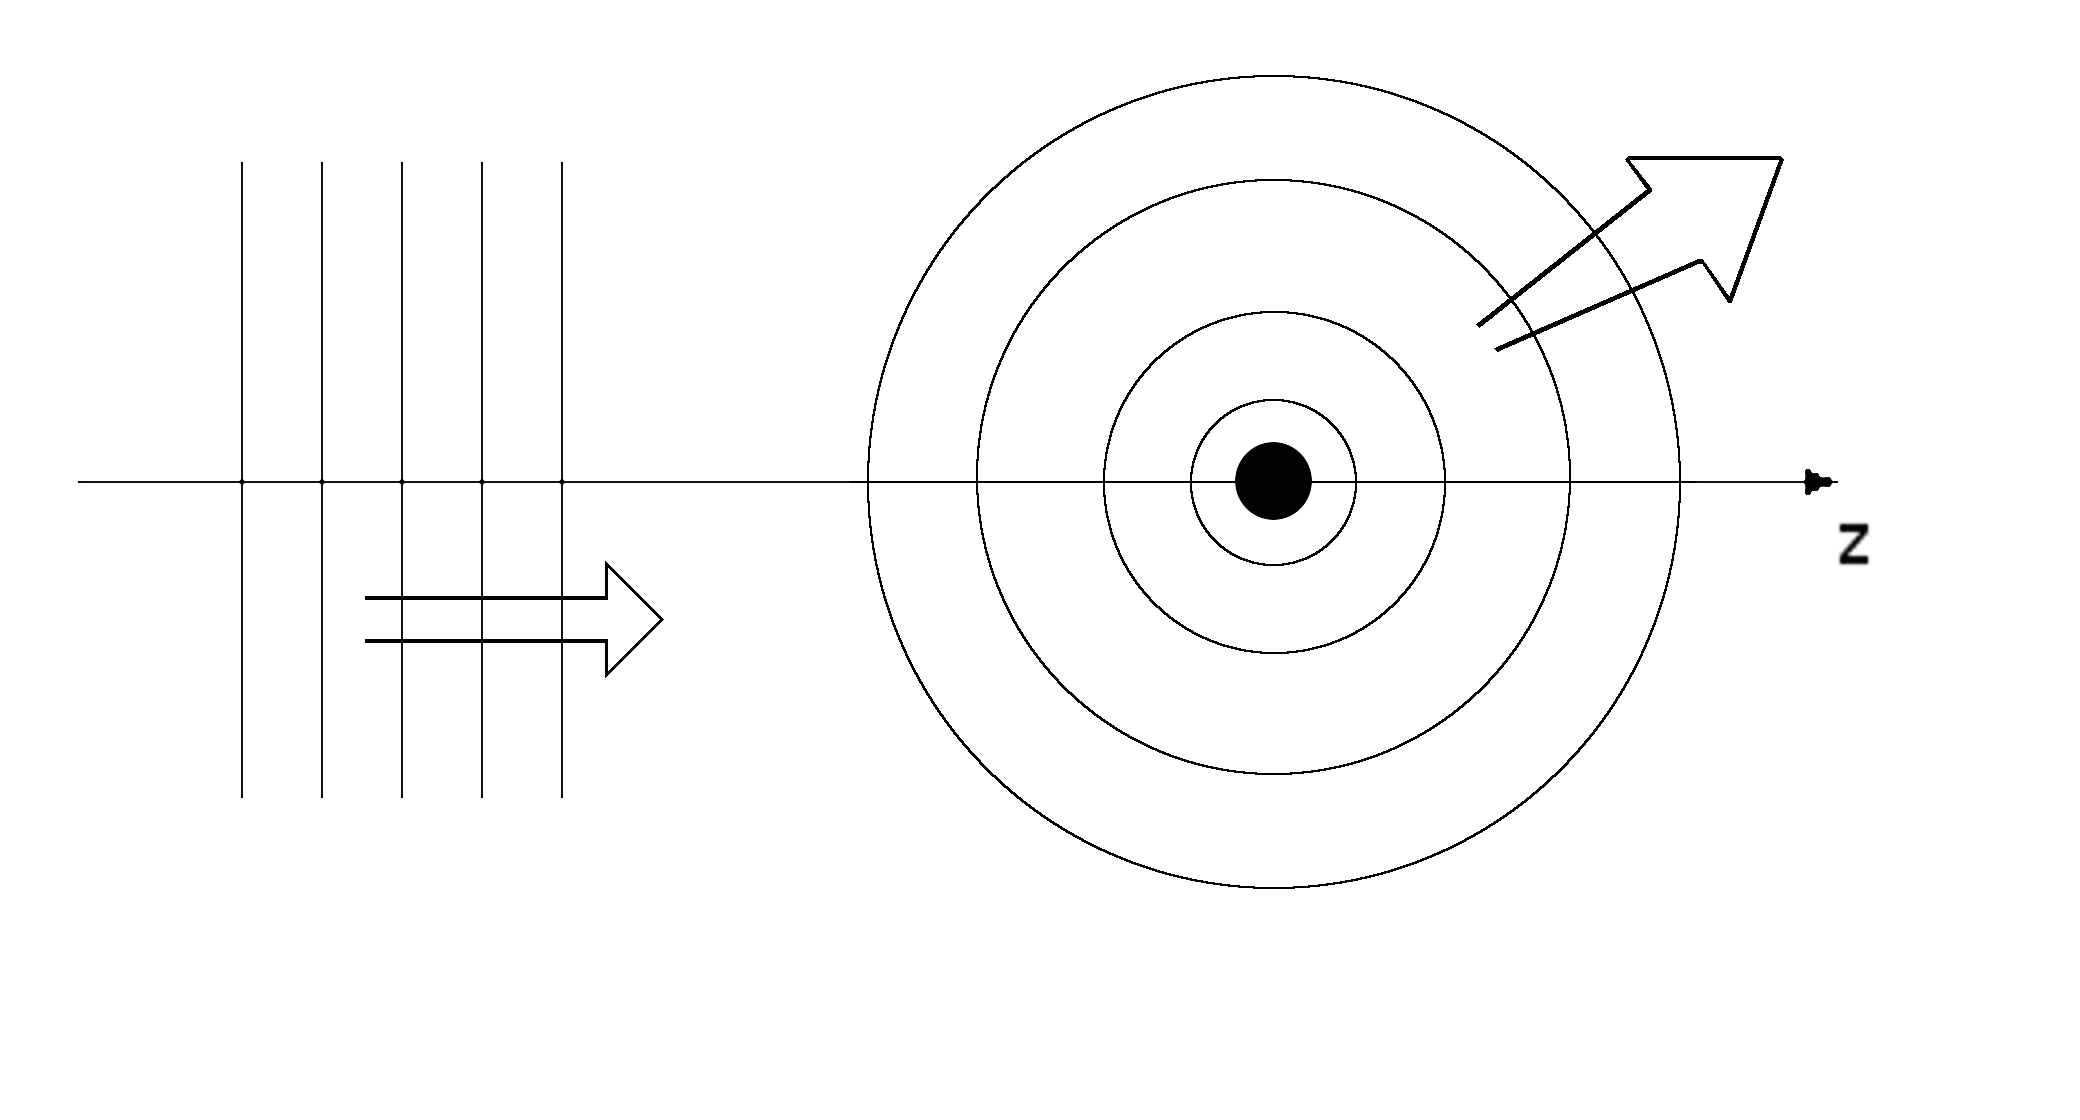
\includegraphics[width=\textwidth]{Figures/scattering_model_2} 
  \caption{Quantum scattering model.}
  \label{fig:qmscatteringmodel}
\end{figure}
Here there is an incoming wave (mathematically represented by $e^{ikz}$) and a spherical wave (represented by $e^{ikr}/r$). $r$ and $z$ are coordinates, $i$ is the imaginary unit, and $k$ is the wave number, classically related to the energy as $k=\sqrt{2mE}/\hbar$. Then basic quantum mechanics suggests that the solution to the Schr\"{o}dinger equation has the form
\begin{equation}
\label{eqn:scatteringwavefunction}
\psi (r,\theta)\approx A \big(e^{ikz}+f(\theta)\frac{e^{ikr}}{r}\big),
\end{equation}
where $A$ is the total amplitude and $f(\theta)$ is the scattering amplitude. The probability of the particle scattering in a particular direction is given by the amplitude squared, $|f(\theta)|^2$, and is the object of this derivation. Now, $\psi$ solves the differential (time-independent) Schr\"{o}dinger equation, which usually has the form
\begin{equation} \nonumber
-\frac{\hbar^2}{2m}\nabla^2\psi+V\psi=E\psi,
\end{equation}
where $V$ is the system potential and $E$ is the energy of the wavefunction. This can be expressed alternatively by assigning $Q\equiv V\psi\cdot{2m}/{\hbar^2}$ and recalling that $k=\sqrt{2mE}/\hbar$. Then
%
\begin{equation}
\label{eqn:schrodinger}
(\nabla^2+k^2)\psi=Q.
\end{equation}

From Eqn. \ref{eqn:scatteringwavefunction} it is clear that it is advantageous to solve Eqn. \ref{eqn:schrodinger} for $\psi$, and if Eqn. \ref{eqn:schrodinger} is solved for $\psi$ then it suggests that $\psi$ will be in integral form (note: it does not matter at this point that $Q$ is a function of $\psi$, since the task will be to compare the integrated solution of Eqn. \ref{eqn:schrodinger} with that of Eqn. \ref{eqn:scatteringwavefunction}). Observe then that Eqn. \ref{eqn:schrodinger} may again be rewritten as
%
\begin{equation} \nonumber
(\nabla^2+k^2)\psi(\vec{r})=Q (\vec{r}) =\int \delta^3(\vec{r}-\vec{r}_0)Q(\vec{r}_0)d^3\vec{r}_0.
\end{equation}
Now it is natural to guess that there exists some function $G(\vec{r})$ such that
%
\begin{equation}
\label{eqn:psigreen}
\psi(\vec{r})=\int G(\vec{r}-\vec{r}_0)Q(\vec{r}_0)d^3\vec{r}_0,
\end{equation}
in which case
%
\begin{equation} \nonumber
(\nabla^2+k^2)\psi(\vec{r})=(\nabla^2+k^2)\int G(\vec{r}-\vec{r}_0)Q(\vec{r}_0) d^3\vec{r}_0
\end{equation}
\begin{equation} \nonumber
=\int \big[(\nabla^2+k^2)G(\vec{r}-\vec{r}_0)\big]Q(\vec{r}_0) d^3\vec{r}_0
\end{equation}
\begin{equation} \nonumber
=\int\delta^3(\vec{r}-\vec{r}_0)Q(\vec{r}_0)d^3\vec{r}_0=Q(\vec{r}),
\end{equation}
and so one comes to the conclusion that
%
\begin{equation}
\label{eqn:helmholtz}
(\nabla^2+k^2)G(\vec{r})=\delta^3(\vec{r}).
\end{equation}
If Eqn. \ref{eqn:helmholtz} seems familiar, it is because this is the Helmholtz equation with a delta function source. $G(\vec{r})$ is Green's function for the Helmholtz equation, and in this case is the response to the delta function source. Now, if one accepts that there exists a well-known particular solution for Eqn. \ref{eqn:helmholtz}, then one could skip forward to the solution in Eqn. \ref{eqn:greensolution}; however, it will also be derived subsequently.

The usual strategy in solving systems like Eqn. \ref{eqn:helmholtz} is to Fourier transform both the Green's function and the delta function. Then creating the dummy variable $\vec{s}$, the transform yields
%
\begin{equation} \nonumber
G(\vec{r})=\frac{1}{(2\pi)^\frac{3}{2}}\int e^{i\vec{s}\cdot\vec{r}} g(\vec{s})d^3\vec{s},
\end{equation}
and
%
\begin{equation} \nonumber
\delta^3(\vec{r})=\frac{1}{(2\pi)^3}\int e^{i\vec{s}\cdot\vec{r}} d^3\vec{s}.
\end{equation}
Then from Eqn. \ref{eqn:helmholtz},
%
\begin{equation} \nonumber
\frac{1}{(2\pi)^\frac{3}{2}}\int (k^2e^{i\vec{s}\cdot\vec{r}}-s^2e^{i\vec{s}\cdot\vec{r}})g(\vec{s})d^3\vec{s}=\frac{1}{(2\pi)^3}\int e^{i\vec{s}\cdot\vec{r}}d^3\vec{s},
\end{equation}
it is clear that $g(\vec{s})=1/(2\pi)^{3/2}(k^2-s^2)$. Now all that is left is to find $G(\vec{r})$ from its transformation:
%
\begin{equation} \nonumber
G(\vec{r})=\frac{1}{(2\pi)^3}\int e^{i\vec{s}\cdot\vec{r}}\frac{d^3\vec{s}}{k^2-s^2}
\end{equation}
%
\begin{equation} \nonumber
G(\vec{r})=\frac{1}{(2\pi)^3}\int_0^\infty \frac{s}{k^2-s^2} \big(\int_0^\pi e^{isr\cos\theta}\sin\theta d\theta\big)ds \int_0^{2\pi}d\phi.
\end{equation}
The integration over $\phi$ is trivial, and the integration over $\theta$ can be done via $u$ substitution. The last integral is over $s$, and is
%
\begin{equation} \nonumber
G(\vec{r})=\frac{1}{2\pi^2r}\int_0^\infty\frac{s\sin{sr}}{k^2-s^2}ds=\frac{1}{4\pi^2r}\int_{-\infty}^\infty\frac{s\sin{sr}}{k^2-s^2}ds.
\end{equation}
This integral is not simple to solve, but it does have two poles at $s=k$ and $s=-k$, which implies the technique of choice should be to use Cauchy's integral formula for simple poles\footnote{This touches an area of mathematics known as the calculus of residues, and is based on the Laurent series.}:
%
\begin{equation}
\label{eqn:cauchy}
\oint \frac{f(z)}{z-z_0}dz=2\pi if(z_0),
\end{equation}
where the integral is done over some path in the complex plane and $z_0$ is the pole of interest which lies in the enclosed path (note: the integral is zero if there exist no poles in the enclosed path). It follows then that $f(z)$ is not simply any function, but a necessarily complex function which is closed. For this reason, the (strictly real) Green's function integral should be split up into two (strictly complex) functions, as depicted by Figure \ref{fig:complexgreen}. This can be done by expanding the $\sin sr$ term and factoring $k^2-s^2$:
%
\begin{equation}
\label{eqn:complexgreen}
G(\vec{r})=\frac{i}{8\pi^2r}\Big[ \int_{-\infty}^\infty \frac{se^{isr}}{(s-k)(s+k)}ds-\int_{-\infty}^\infty \frac{se^{-isr}}{(s-k)(s+k)}ds \Big].
\end{equation}
%
\begin{figure}
  \centering
    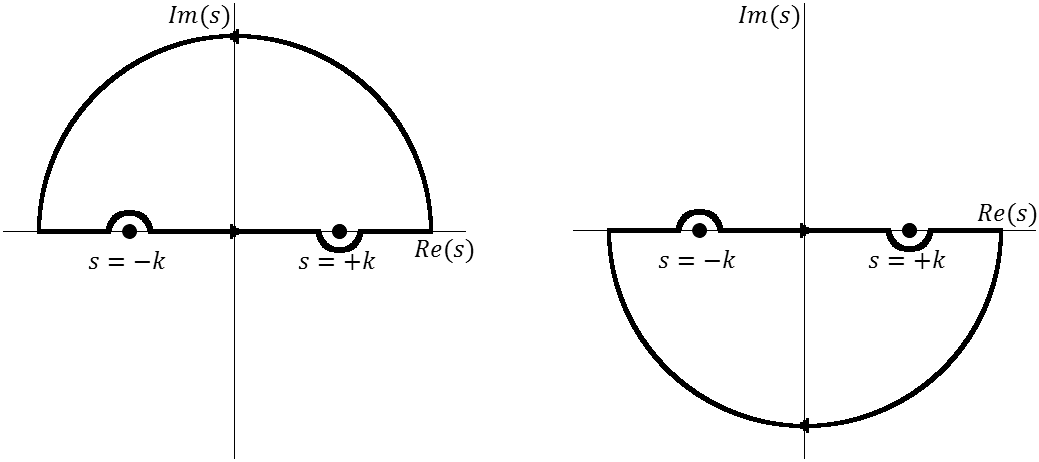
\includegraphics[width=\textwidth]{Figures/complexgreen} 
  \caption{Two parts of Green's function with their poles at $s=\pm k$, altered to be closed via semicircle at $|s|=\pm\infty$.}
  \label{fig:complexgreen}
\end{figure}

Observe that in Eqn. \ref{eqn:complexgreen} the path integrals at $|s|=\pm\infty$ have been left out. This is because they do not contribute to the integral, since the first integrand corresponds to the left side of Figure \ref{fig:complexgreen} and goes like $e^{isr}$, hence going to zero at large positive imaginary numbers. Similarly, the second integrand goes like $e^{-isr}$ and goes to zero at large negative imaginary numbers.

Combining Eqns. \ref{eqn:cauchy} and \ref{eqn:complexgreen}, it can be seen that
%
\begin{equation}
\nonumber
G(\vec{r})=\frac{i}{8\pi^2r}[(i\pi e^{ikr})-(-i\pi e^{ikr})]=-\frac{e^{ikr}}{4\pi r}.
\end{equation}
This is a particular solution to the Helmholtz equation. To get a general solution, the solution to the homogeneous Helmholtz equation must be added:
%
\begin{equation}
\label{eqn:greensolution}
G(\vec{r})=G_0(\vec{r})-\frac{e^{ikr}}{4\pi r};
\end{equation}
that is, $G_0(\vec{r})$ solves $(\nabla^2+k^2)G_0(\vec{r})=0$.

Using Eqn. \ref{eqn:psigreen} in conjunction with Eqn. \ref{eqn:greensolution} gives rise to the \emph{integrated} time-independent Schr\"{o}dinger equation:
%
\begin{equation} \label{eqn:integratedschrodinger}
\psi(\vec{r})=\psi_0 (\vec{r})-\frac{m}{2\pi\hbar^2}\int\frac{e^{ik|\vec{r}-\vec{r}_0|}}{|\vec{r}-\vec{r}_0|}V(\vec{r}_0)\psi(\vec{r}_0)d^3\vec{r}_0.
\end{equation}
%
Eqn. \ref{eqn:integratedschrodinger} gives the recursive form for $\psi$. Let $g=-me^{ik|\vec{r}-\vec{r}_0|}/2\pi\hbar^2|\vec{r}-\vec{r}_0|$. Then Eqn. \ref{eqn:integratedschrodinger} says that
%
\begin{equation} \nonumber
\psi=\psi_0+\int gV\psi = \psi_0+\int gV (\psi_0+\int gV\psi).
\end{equation}
%
Applying this recursion several times gives the Born series:
%
\begin{equation}\nonumber
\psi=\psi_0+\int gV\psi_0+\int \int gVgV\psi_0 + \int \int \int gVgVgV\psi_0 + ...
\end{equation}
%
The zeroth term is exact if there is no scattering whatsoever (i.e. $V=0$) and the first term is accurate if the scattering potential is weak. For the purposes of this derivation, first order will be a sufficient approximation for $\psi$. Then
%
\begin{equation} \nonumber
\psi=\psi_0+\frac{m}{2\pi\hbar^2}\int\frac{e^{ik|\vec{r}-\vec{r}_0}}{|\vec{r}-\vec{r}_0|}V(\vec{r}_0)\psi_0(\vec{r}_0) d^3\vec{r}_0
\end{equation}

Recall that the strategy was to compare this solution of the Helmholtz equation with the wavefunction from the quantum scattering model (Eqn. \ref{eqn:scatteringwavefunction}) in order to find the scattering amplitude, $f(\theta)$. Doing so yields
%
\begin{equation} \nonumber
f(\theta)=-\frac{r}{e^{ikr}}\frac{m}{2\pi\hbar^2A}\int\frac{e^{ik|\vec{r}-\vec{r}_0|}}{|\vec{r}-\vec{r}_0|}V(\vec{r}_0)\psi_0(\vec{r}_0)d^3\vec{r}_0.
\end{equation}
%

The Coulomb potential goes as $1/r^2$, and as such $V(\vec{r}_0)$ is localized about $\vec{r}_0=0$. Since particles are observed far away from their scattering centers, it is advantageous to make use of the fact that $\vec{r} \gg \vec{r}_0$. However, caution must be taken, since one must evaluate the exponential and non-exponential terms separately, for they are of separate orders. For the non-exponential terms, this is simple, since
%
\begin{equation}\nonumber
\frac{r}{|\vec{r}-\vec{r}_0|}\approx1.
\end{equation}
%
The exponential terms look like
%
\begin{equation}\nonumber
e^{ik(|\vec{r}-\vec{r}_0|-r)},
\end{equation}
and so it is useful to expand the absolute value as
\begin{equation}\nonumber
|\vec{r}-\vec{r}_0|^2=r^2+r_0^2-2\vec{r}\cdot\vec{r}_0\approx r^2(1-2\frac{\vec{r}\cdot\vec{r}_0}{r^2}),
\end{equation}
%
or simply
%
\begin{equation} \nonumber |\vec{r}-\vec{r}_0|\approx r-\hat{r}\cdot\vec{r}_0. \end{equation}
%
This leaves
%
\begin{equation} \label{eqn:generalscattering}
f(\theta)=\frac{m}{2\pi\hbar^2}\int
e^{-ik\hat{r}\cdot\vec{r}_0}
V(\vec{r}_0)
e^{ik\hat{z}\cdot\vec{r}_0}
d^3\vec{r}_0,
\end{equation}
%
where $\psi_0(\vec{r}_0)=Ae^{ik\hat{z}\cdot\vec{r}_0}$.
Now define $\vec{\kappa}\equiv k(\hat{z}-\hat{r})$ such that $\kappa=2k\sin{\theta/2}$. The exponential term becomes
%
\begin{equation} \nonumber
e^{i\vec{\kappa}\cdot\vec{r}_0}=e^{i\kappa r_0\cos{\theta_0}}.
\end{equation}
Furthermore, the form of the potential $V$ is known. Since the scattering for the low Z target happens at low temperatures, it is possible to use the Fermi-Thomas approximation for screening \cite{ashcroft}. This modifies the first Maxwell equation to
\begin{equation} \nonumber
(\nabla^2-b^2)V(r)=-\frac{Q}{\epsilon_0}\delta(r),
\end{equation}
%
which has the solution
\begin{equation} \nonumber
V(r)=\frac{Q}{4\pi\epsilon_0}\frac{e^{-br}}{r},
\end{equation}
where $b$ is some constant, $\epsilon_0$ is the permittivity of free space, and $Q$ is the charge of the potential (in this case, the atomic number $Z$). Then the quantum scattering equation (Eqn. \ref{eqn:generalscattering}) becomes
%
\begin{equation} \nonumber
f(\theta)\propto \int e^{i\kappa r_0\cos(\theta_0)}e^{-br_0}r_0\sin(\theta_0)dr_0 d\theta_0 d\phi_0,
\end{equation}
where the amplitude terms have been left out since $|f(\theta)|^2$ is normalized anyway. Here it is seen that there does exist some $\theta$ dependence in $f(\theta)$ (by virtue of $\kappa$). The integral over $\phi_0$ is trivial, and the integral over $\theta_0$ can be done via $u$ substitution. This leaves
\begin{equation} \nonumber
f(\theta)\propto \frac{1}{\kappa}\int_0^\infty e^{-br_0}\sin(\kappa r_0) dr_0,
\end{equation}
%
which has the solution
\begin{equation}\nonumber
f(\theta)\propto\frac{1}{b^2+\kappa^2}.
\end{equation}
For classical Rutherford scattering, $b\rightarrow 0$. Recalling that $\kappa=2k\sin{\theta/2}$ yields the final Rutherford scattering distribution:
\begin{equation}
\label{eqn:rutherford}
|f(\theta)|^2\propto \frac{1}{\sin^4(\theta/2)}\propto\frac{1}{(1-\cos^2{\theta})^2}.
\end{equation}

Only the tail of Eqn. \ref{eqn:rutherford} should be used since it blows up at $\theta=0$. This may seem like a contradiction, since the Born series was truncated at the weak potential term (the first nontrivial term), and hence the incoming muons should not scatter much at all! In fact, the muons are not scattering much at all for each individual atom they encounter. Over the entire absorber, however, some muons will have a net scattering angle which is small (and therefore should not be approximated by the Rutherford tail) whereas others will have a large net scattering angle (and are well represented by Eqn. \ref{eqn:rutherford}). Many weak potentials can still induce a relatively large scattered angle.
